\chapter{Result and Discussion}
In this chapter, we discuss about the results obtained through data analysis.
\section{Inclusive Cross Section}

\section{Neutron Removal Cross Section}
\begin{table}[h]
\centering
\begin{tabular}{c|c|c|c}
    \hline
    & $\sigma_{incl}$ (mb) & $\sigma_{-2n}$ (mb) & $\sigma_{-4n}$ (mb) \\
    \hline \hline
    $^{17}$B + Pb&  & 713() &    \\ 
    $^{17}$B + C &  & 149() &   \\ 
    $\sigma_{Pb}/\sigma_{C}$ &  &  &    \\ \hline
\end{tabular}
\caption{Reaction Cross Section of Boron Isotopes}
\label{tab:Reaction Cross Section of Boron Isotopes}

\end{table}

\section{Relative Energy Spectrum}

\section{Coulomb Dissociation Cross Section}
Coulomb dissociation cross section can be extracted by using the following equation.
\begin{align}
\sigma_{CD} = \sigma_{incl}(Pb) - \Gamma \sigma_{incl}(C)
\end{align}
We used $\Gamma$ value from calculation . 

\begin{table}[h]
\centering
    \begin{tabular}{c|c|c}
        \hline
        & $\Gamma$ & $\sigma_{coul}$   \\
        \hline
        $^{17}$B& 2.385 &   281 $\pm$ 8 mb \\ 
        \hline
    \end{tabular}
\caption{Coulomb Dissociation Cross Section}
\label{Coulomb Dissociation Cross Section}
\end{table}

\begin{center}
    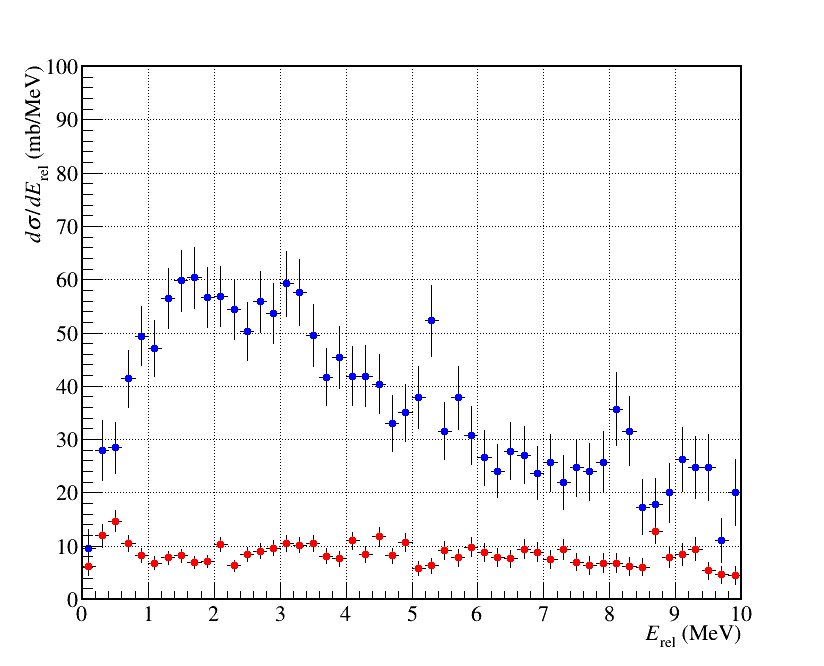
\includegraphics[width=13cm]{chapter5/coulomb_pb_c.png}    
    \captionof{figure}{Cross Section}
    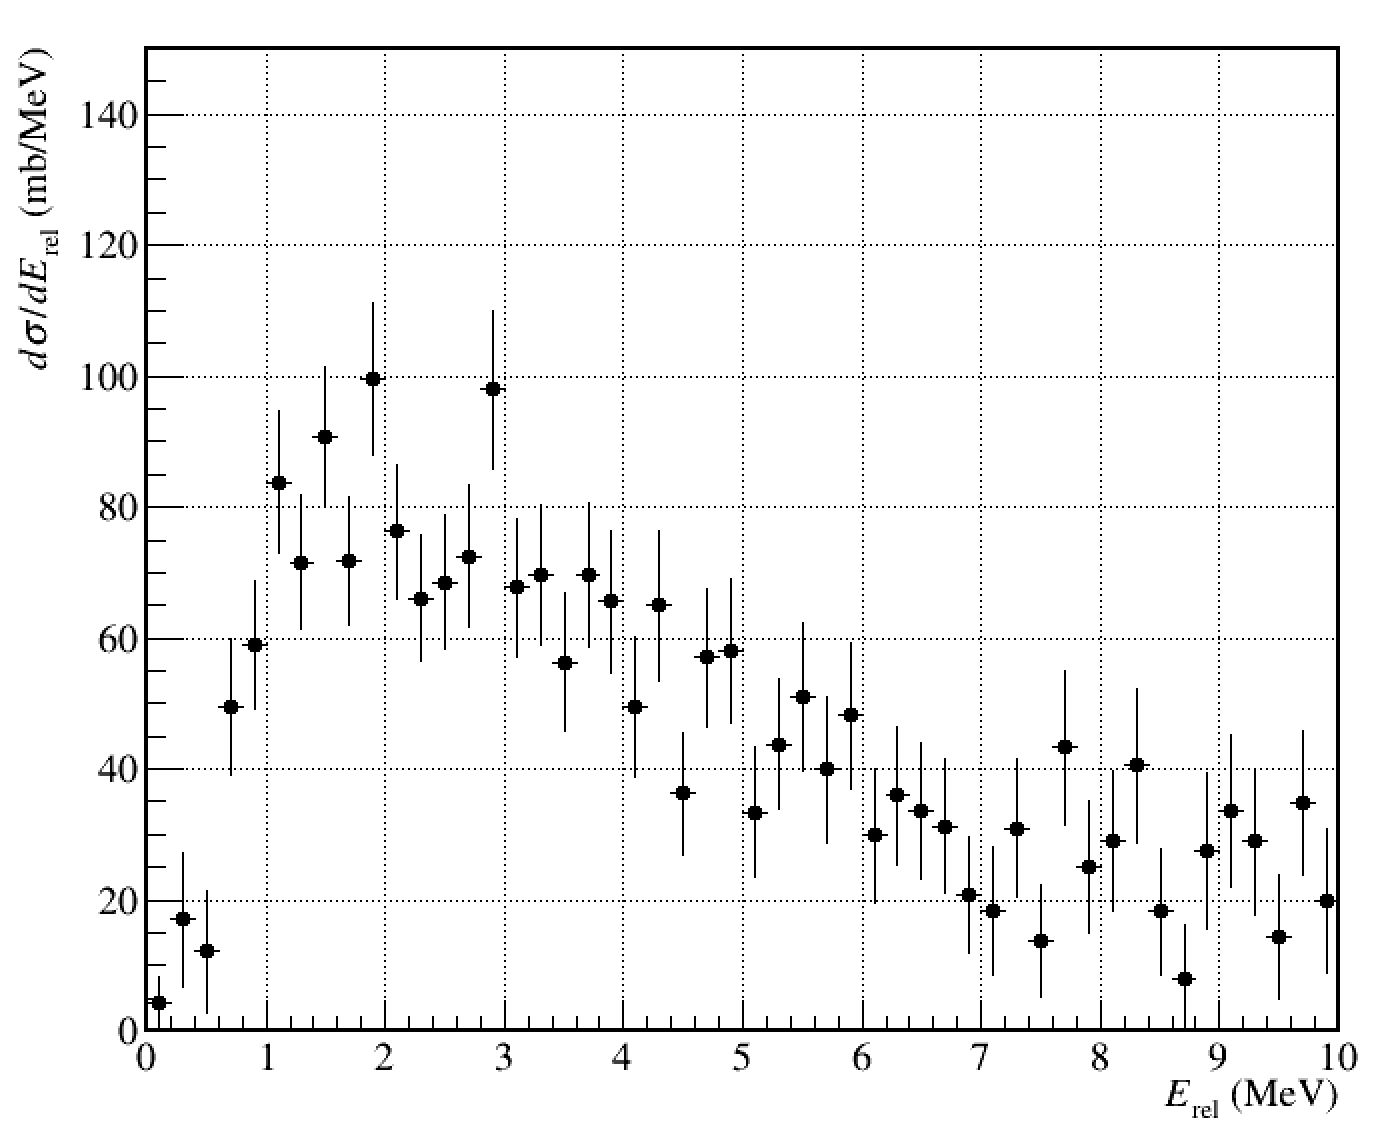
\includegraphics[width=13cm]{chapter5/dsigmadE.png}    
    \captionof{figure}{Coulomb Dissociation Cross Section}
\end{center}    

About reduced dipole transition probability, we can extract $B(E1)$ strength as follows.
\begin{align}
    \frac{d \sigma_{coul}}{dE_x} = \frac{16 \pi^{3} }{9 \hbar c} N_{\text{E1}}(E_x) \frac{dB(\text{E1})}{dE_x}
\end{align}

\begin{center}
    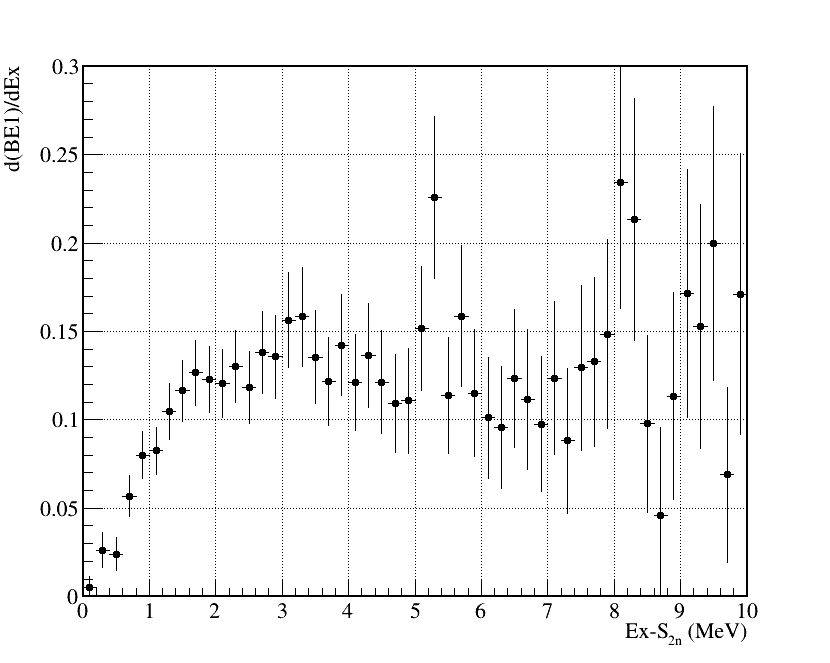
\includegraphics[width=13cm]{chapter5/dBdEx.png}    
    \captionof{figure}{B(E1) Strength}
\end{center}  
\begin{align}
    B(E1) &= \int_{0}^{+\inf} \frac{dB(E1)}{dE_x} dE_x \\
          &= \int_{0}^{+10} \frac{dB(E1)}{dE_x} dE_x \\ 
          &= 1.22 \pm 0.06  [e^{2}fm^{2}]    
\end{align}  

\section{Dineutron Correlation}

\begin{align}
    B(E1) = \frac{3}{\pi} \bigg( \frac{Ze}{A} \bigg)^2 \langle r^{2}_{c-nn} \rangle
\end{align}
With the obtained $B(E1)$ strength up to 10 MeV, we can extract $\sqrt{ \langle r^{2}_{c-nn} \rangle}$ as follows.
\begin{align}
    \sqrt{ \langle r^{2}_{c-nn} \rangle} = 0.00 \pm 0.00 (stat.) \pm 0.00 (syst.) \text{ fm}
\end{align}
Furthermore, we can extract the distance of $2n$ from three body model.
\begin{align}
    \langle r^{2}_{halo} \rangle = \frac{A_c}{A} \langle r^{2}_{core} \rangle + \frac{2A_c}{A^2} \langle r^{2}_{c-nn} \rangle - \frac{1}{2A} \langle r^{2}_{nn} \rangle
\end{align}
where $A$ and $A_c$ is the mass number of halo nucleus and core. $\langle r^{2}_{h} \rangle$ and $\langle r^{2}_{c} \rangle$ are the mean-square matter radius of halo nuclei and the core, which is 3.00(6) fm and 2.75(6) fm respectively.
\begin{align}
    \sqrt{ \langle r^{2}_{nn} \rangle} = 3.20 \pm 0.00 (stat.) \pm 0.00 (syst.) \text{ fm}
\end{align}
Finally, the mean opening angle of dineutron can be extracted as follows.
\begin{align}
    \langle \theta_{nn} \rangle = 6.57 \pm 0.00 (stat.) \pm 0.00 (syst.) \text{ deg.}
\end{align}